\itemhead{习题4.2 · 第15题（教材p.114）}{XJ-B1-C04-HW-P114-Y1507}
\label{XJ-B1-C04-HW-P114-Y1507}
{\footnotesize 湘教版教材p.114 / PDF第121页 / 习题4.2 / 第15题}
\field{原题}{函数 $y=3a^x$ 的图象与函数 $y=a^x$ 的图象有什么相同点和不同点？函数 $y=-2a^x$ 呢？思考后画图检验。}
\field{参考答案}{三者定义域均为 $\mathbb R$。$3a^x$ 与 $a^x$ 同增减、值域均为 $(0,+\infty)$，纵坐标扩大3倍，定点由 $(0,1)$ 变 $(0,3)$；$-2a^x$ 的值域为 $(-\infty,0)$，关于 $x$ 轴翻折再纵向扩大2倍，增减方向相反，定点 $(0,-2)$。三者均非奇非偶；是否是标准指数函数与是否有指数型性质要区分。}
\begin{center}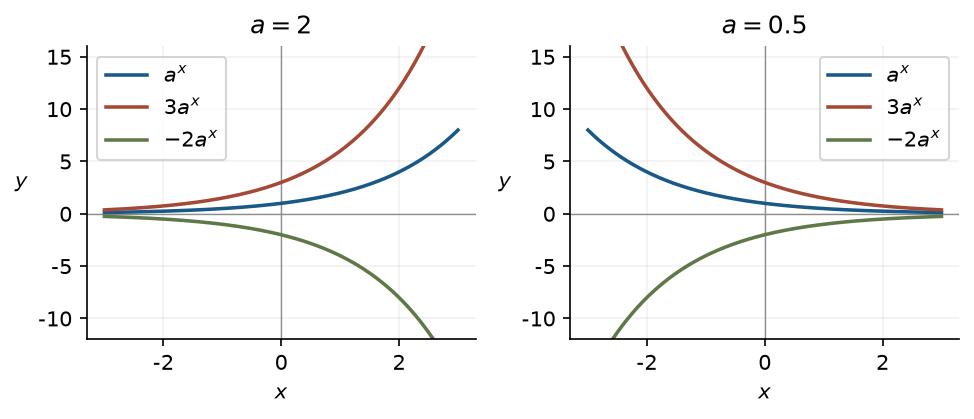
\includegraphics[width=.84\linewidth,height=.38\textheight,keepaspectratio]{figures/C04-HW114-15.png}\end{center}
{\small \field{关联知识}{E01 指数函数的概念、图象与性质（教材帮p.150、151 / PDF159、160）；F09 图象平移、伸缩与对称（教材帮p.86、94 / PDF95、103）}
\field{方法与易错点}{先查底数条件，利用已知点定底数，再据单调性及图象求值或范围。 易错：只要求底数非负；漏排1；将 $a^x+b$ 当标准指数函数且仍用原值域。}
\field{答案依据}{答案册相关题组：PDF第32页（册内页31）；按当前题库原题逐项重算，不按旧版题号机械对套。}}
